\documentclass[twoside]{book}

% Packages required by doxygen
\usepackage{fixltx2e}
\usepackage{calc}
\usepackage{doxygen}
\usepackage[export]{adjustbox} % also loads graphicx
\usepackage{graphicx}
\usepackage[utf8]{inputenc}
\usepackage{makeidx}
\usepackage{multicol}
\usepackage{multirow}
\PassOptionsToPackage{warn}{textcomp}
\usepackage{textcomp}
\usepackage[nointegrals]{wasysym}
\usepackage[table]{xcolor}

% Font selection
\usepackage[T1]{fontenc}
\usepackage[scaled=.90]{helvet}
\usepackage{courier}
\usepackage{amssymb}
\usepackage{sectsty}
\renewcommand{\familydefault}{\sfdefault}
\allsectionsfont{%
  \fontseries{bc}\selectfont%
  \color{darkgray}%
}
\renewcommand{\DoxyLabelFont}{%
  \fontseries{bc}\selectfont%
  \color{darkgray}%
}
\newcommand{\+}{\discretionary{\mbox{\scriptsize$\hookleftarrow$}}{}{}}

% Page & text layout
\usepackage{geometry}
\geometry{%
  a4paper,%
  top=2.5cm,%
  bottom=2.5cm,%
  left=2.5cm,%
  right=2.5cm%
}
\tolerance=750
\hfuzz=15pt
\hbadness=750
\setlength{\emergencystretch}{15pt}
\setlength{\parindent}{0cm}
\setlength{\parskip}{3ex plus 2ex minus 2ex}
\makeatletter
\renewcommand{\paragraph}{%
  \@startsection{paragraph}{4}{0ex}{-1.0ex}{1.0ex}{%
    \normalfont\normalsize\bfseries\SS@parafont%
  }%
}
\renewcommand{\subparagraph}{%
  \@startsection{subparagraph}{5}{0ex}{-1.0ex}{1.0ex}{%
    \normalfont\normalsize\bfseries\SS@subparafont%
  }%
}
\makeatother

% Headers & footers
\usepackage{fancyhdr}
\pagestyle{fancyplain}
\fancyhead[LE]{\fancyplain{}{\bfseries\thepage}}
\fancyhead[CE]{\fancyplain{}{}}
\fancyhead[RE]{\fancyplain{}{\bfseries\leftmark}}
\fancyhead[LO]{\fancyplain{}{\bfseries\rightmark}}
\fancyhead[CO]{\fancyplain{}{}}
\fancyhead[RO]{\fancyplain{}{\bfseries\thepage}}
\fancyfoot[LE]{\fancyplain{}{}}
\fancyfoot[CE]{\fancyplain{}{}}
\fancyfoot[RE]{\fancyplain{}{\bfseries\scriptsize Generated by Doxygen }}
\fancyfoot[LO]{\fancyplain{}{\bfseries\scriptsize Generated by Doxygen }}
\fancyfoot[CO]{\fancyplain{}{}}
\fancyfoot[RO]{\fancyplain{}{}}
\renewcommand{\footrulewidth}{0.4pt}
\renewcommand{\chaptermark}[1]{%
  \markboth{#1}{}%
}
\renewcommand{\sectionmark}[1]{%
  \markright{\thesection\ #1}%
}

% Indices & bibliography
\usepackage{natbib}
\usepackage[titles]{tocloft}
\setcounter{tocdepth}{3}
\setcounter{secnumdepth}{5}
\makeindex

% Custom commands
\newcommand{\clearemptydoublepage}{%
  \newpage{\pagestyle{empty}\cleardoublepage}%
}

\usepackage{caption}
\captionsetup{labelsep=space,justification=centering,font={bf},singlelinecheck=off,skip=4pt,position=top}

%===== C O N T E N T S =====

\begin{document}

% Titlepage & ToC
\pagenumbering{alph}
\begin{titlepage}
\vspace*{7cm}
\begin{center}%
{\Large Vectorial\+O\+DE \\[1ex]\large {\tt https\+://c4science.\+ch/source/\+Group15/repository/master/} }\\
\vspace*{1cm}
{\large Generated by Doxygen 1.8.14}\\
\end{center}
\end{titlepage}
\clearemptydoublepage
\pagenumbering{roman}
\tableofcontents
\clearemptydoublepage
\pagenumbering{arabic}

%--- Begin generated contents ---
\chapter{Hierarchical Index}
\section{Class Hierarchy}
This inheritance list is sorted roughly, but not completely, alphabetically\+:\begin{DoxyCompactList}
\item \contentsline{section}{Input}{\pageref{class_input}}{}
\item \contentsline{section}{Solution}{\pageref{class_solution}}{}
\item \contentsline{section}{Vectorial\+O\+DE}{\pageref{class_vectorial_o_d_e}}{}
\begin{DoxyCompactList}
\item \contentsline{section}{Bashforth}{\pageref{class_bashforth}}{}
\begin{DoxyCompactList}
\item \contentsline{section}{Bashforth\+First\+Step}{\pageref{class_bashforth_first_step}}{}
\item \contentsline{section}{Bashforth\+Fourth\+Step}{\pageref{class_bashforth_fourth_step}}{}
\item \contentsline{section}{Bashforth\+Second\+Step}{\pageref{class_bashforth_second_step}}{}
\item \contentsline{section}{Bashforth\+Third\+Step}{\pageref{class_bashforth_third_step}}{}
\end{DoxyCompactList}
\item \contentsline{section}{Runge\+Kutta}{\pageref{class_runge_kutta}}{}
\begin{DoxyCompactList}
\item \contentsline{section}{Runge\+Kutta\+Order2}{\pageref{class_runge_kutta_order2}}{}
\item \contentsline{section}{Runge\+Kutta\+Order4}{\pageref{class_runge_kutta_order4}}{}
\end{DoxyCompactList}
\end{DoxyCompactList}
\end{DoxyCompactList}

\chapter{Class Index}
\section{Class List}
Here are the classes, structs, unions and interfaces with brief descriptions\+:\begin{DoxyCompactList}
\item\contentsline{section}{\textbf{ Bashforth} \\*Class allowing a more precise definition of one of the O\+DE solvers technics which is Adam-\/\+Bashforth method. This is an abstract class as before because the method Solve\+Vectorial\+O\+DE is virtual and it will be defined in different ways in the inherited classes. The different Adam-\/\+Bashforth method correspond to the different order we use to solve the system }{\pageref{class_bashforth}}{}
\item\contentsline{section}{\textbf{ Bashforth\+First\+Step} \\*Class implementing the Adam-\/\+Bashforth 1 step (Forward Euler) to solve the O\+DE system. \doxyref{Bashforth}{p.}{class_bashforth} method allows the solving of the O\+DE system. This class is implementing in such a way that it only writes the solution every Write\+Output\+Timestep. This class is inherited from \doxyref{Bashforth}{p.}{class_bashforth} class also inherited from \doxyref{Vectorial\+O\+DE}{p.}{class_vectorial_o_d_e} }{\pageref{class_bashforth_first_step}}{}
\item\contentsline{section}{\textbf{ Bashforth\+Fourth\+Step} \\*Class implementing the Adam-\/\+Bashforth 4 steps to solve the O\+DE system. \doxyref{Bashforth}{p.}{class_bashforth} method allows the solving of the O\+DE system. This class is implementing in such a way that it only writes the solution every Write\+Output\+Timestep. This class is inherited from \doxyref{Bashforth}{p.}{class_bashforth} class also inherited from \doxyref{Vectorial\+O\+DE}{p.}{class_vectorial_o_d_e} }{\pageref{class_bashforth_fourth_step}}{}
\item\contentsline{section}{\textbf{ Bashforth\+Second\+Step} \\*Class implementing the Adam-\/\+Bashforth 2 steps to solve the O\+DE system. \doxyref{Bashforth}{p.}{class_bashforth} method allows the solving of the O\+DE system. This class is implementing in such a way that it only writes the solution every Write\+Output\+Timestep. This class is inherited from \doxyref{Bashforth}{p.}{class_bashforth} class also inherited from \doxyref{Vectorial\+O\+DE}{p.}{class_vectorial_o_d_e} }{\pageref{class_bashforth_second_step}}{}
\item\contentsline{section}{\textbf{ Bashforth\+Third\+Step} \\*Class implementing the Adam-\/\+Bashforth 3 steps to solve the O\+DE system. \doxyref{Bashforth}{p.}{class_bashforth} method allows the solving of the O\+DE system. This class is implementing in such a way that it only writes the solution every Write\+Output\+Timestep. This class is inherited from \doxyref{Bashforth}{p.}{class_bashforth} class also inherited from \doxyref{Vectorial\+O\+DE}{p.}{class_vectorial_o_d_e} }{\pageref{class_bashforth_third_step}}{}
\item\contentsline{section}{\textbf{ Input} \\*Class allowing the saving of all the variables to define the system we want to solve. In fact, it takes as input variable (integer or double)\+: Timestep, Dimension, Order, Number\+Steps, Write\+Output\+Timestep. Moreover, \doxyref{Input}{p.}{class_input} object needs 3 matrix to define the system \+: Initial\+Condition\+Matrix, Coefficient\+Matrix, Function\+Matrix. Matrix are defined to be vector of vector of double. \doxyref{Input}{p.}{class_input} variables are given to the input class by the constructor. The other methods are getter allowing the access to theses private attributes }{\pageref{class_input}}{}
\item\contentsline{section}{\textbf{ Runge\+Kutta} \\*Class allowing a more precise definition of one of the O\+DE solvers technics which is Runge-\/\+Kutta method. This is an abstract class as before because the method Solve\+Vectorial\+O\+DE is virtual and it will be defined in different ways in the inherited classes. The different Runge-\/\+Kutta method correspond to the different order we use to solve the system }{\pageref{class_runge_kutta}}{}
\item\contentsline{section}{\textbf{ Runge\+Kutta\+Order2} \\*Class implementing the Runge-\/\+Kutta 2 steps to solve the O\+DE system. Runge-\/\+Kutta method allows the solving of the O\+DE system. This class is implementing in such a way that it only writes the solution every Write\+Output\+Timestep. This class is inherited from \doxyref{Runge\+Kutta}{p.}{class_runge_kutta} class also inherited from \doxyref{Vectorial\+O\+DE}{p.}{class_vectorial_o_d_e} }{\pageref{class_runge_kutta_order2}}{}
\item\contentsline{section}{\textbf{ Runge\+Kutta\+Order4} \\*Class implementing the Runge-\/\+Kutta 4 steps to solve the O\+DE system. Runge-\/\+Kutta method allows the solving of the O\+DE system. This class is implementing in such a way that it only writes the solution every Write\+Output\+Timestep. This class is inherited from \doxyref{Runge\+Kutta}{p.}{class_runge_kutta} class also inherited from \doxyref{Vectorial\+O\+DE}{p.}{class_vectorial_o_d_e} }{\pageref{class_runge_kutta_order4}}{}
\item\contentsline{section}{\textbf{ Solution} \\*This class allows the saving in the memory and the writing in a output file of the solution of the O\+DE system. The constructor need the input object defining the system to create a consistent format for the solution. In this class, method allowing the retrieve, the modification and the writing of the solution are implemented. The attributes of this class are the the solution matrix and two integer defining the size of this solution }{\pageref{class_solution}}{}
\item\contentsline{section}{\textbf{ Vectorial\+O\+DE} \\*Class allowing the definition O\+DE solvers. This is an abstract class. The method Solve\+Vectorial\+O\+DE is virtual and it will be defined in different ways in the inherited classes }{\pageref{class_vectorial_o_d_e}}{}
\end{DoxyCompactList}

\chapter{Class Documentation}
\section{Bashforth Class Reference}
\label{class_bashforth}\index{Bashforth@{Bashforth}}


Class allowing a more precise definition of one of the O\+DE solvers technics which is Adam-\/\+Bashforth method. This is an abstract class as before because the method Solve\+Vectorial\+O\+DE is virtual and it will be defined in different ways in the inherited classes. The different Adam-\/\+Bashforth method correspond to the different order we use to solve the system.  




{\ttfamily \#include $<$Bashforth.\+h$>$}

Inheritance diagram for Bashforth\+:\begin{figure}[H]
\begin{center}
\leavevmode
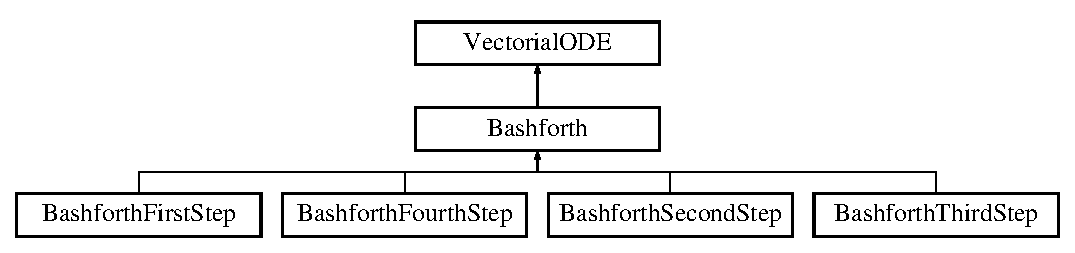
\includegraphics[height=2.957747cm]{class_bashforth}
\end{center}
\end{figure}
\subsection*{Public Member Functions}
\begin{DoxyCompactItemize}
\item 
\textbf{ Bashforth} (\textbf{ Input} \&input, \textbf{ Solution} \&solution)
\begin{DoxyCompactList}\small\item\em Constructor inherited from the \doxyref{Vectorial\+O\+DE}{p.}{class_vectorial_o_d_e} class. \end{DoxyCompactList}\item 
\mbox{\label{class_bashforth_a48d3c2ffe153668992b6e8b79401ac87}} 
virtual void {\bfseries Solve\+Vectorial\+O\+DE} ()=0
\end{DoxyCompactItemize}
\subsection*{Additional Inherited Members}


\subsection{Detailed Description}
Class allowing a more precise definition of one of the O\+DE solvers technics which is Adam-\/\+Bashforth method. This is an abstract class as before because the method Solve\+Vectorial\+O\+DE is virtual and it will be defined in different ways in the inherited classes. The different Adam-\/\+Bashforth method correspond to the different order we use to solve the system. 

\subsection{Constructor \& Destructor Documentation}
\mbox{\label{class_bashforth_ab53efe42b59a80a51731b67ee982f71c}} 
\index{Bashforth@{Bashforth}!Bashforth@{Bashforth}}
\index{Bashforth@{Bashforth}!Bashforth@{Bashforth}}
\subsubsection{Bashforth()}
{\footnotesize\ttfamily Bashforth\+::\+Bashforth (\begin{DoxyParamCaption}\item[{\textbf{ Input} \&}]{input,  }\item[{\textbf{ Solution} \&}]{solution }\end{DoxyParamCaption})}



Constructor inherited from the \doxyref{Vectorial\+O\+DE}{p.}{class_vectorial_o_d_e} class. 


\begin{DoxyParams}{Parameters}
{\em input} & \+: \doxyref{Input}{p.}{class_input} object containing all variables needed to solve the O\+DE. \\
\hline
{\em solution} & \+: Output object where we will store the solution. \\
\hline
\end{DoxyParams}


The documentation for this class was generated from the following files\+:\begin{DoxyCompactItemize}
\item 
Bashforth.\+h\item 
Bashforth.\+cpp\end{DoxyCompactItemize}

\section{Bashforth\+First\+Step Class Reference}
\label{class_bashforth_first_step}\index{Bashforth\+First\+Step@{Bashforth\+First\+Step}}


Class implementing the Adam-\/\+Bashforth 1 step (Forward Euler) to solve the O\+DE system. \doxyref{Bashforth}{p.}{class_bashforth} method allows the solving of the O\+DE system. This class is implementing in such a way that it only writes the solution every Write\+Output\+Timestep. This class is inherited from \doxyref{Bashforth}{p.}{class_bashforth} class also inherited from \doxyref{Vectorial\+O\+DE}{p.}{class_vectorial_o_d_e}.  




{\ttfamily \#include $<$Bashforth\+First\+Step.\+h$>$}

Inheritance diagram for Bashforth\+First\+Step\+:\begin{figure}[H]
\begin{center}
\leavevmode
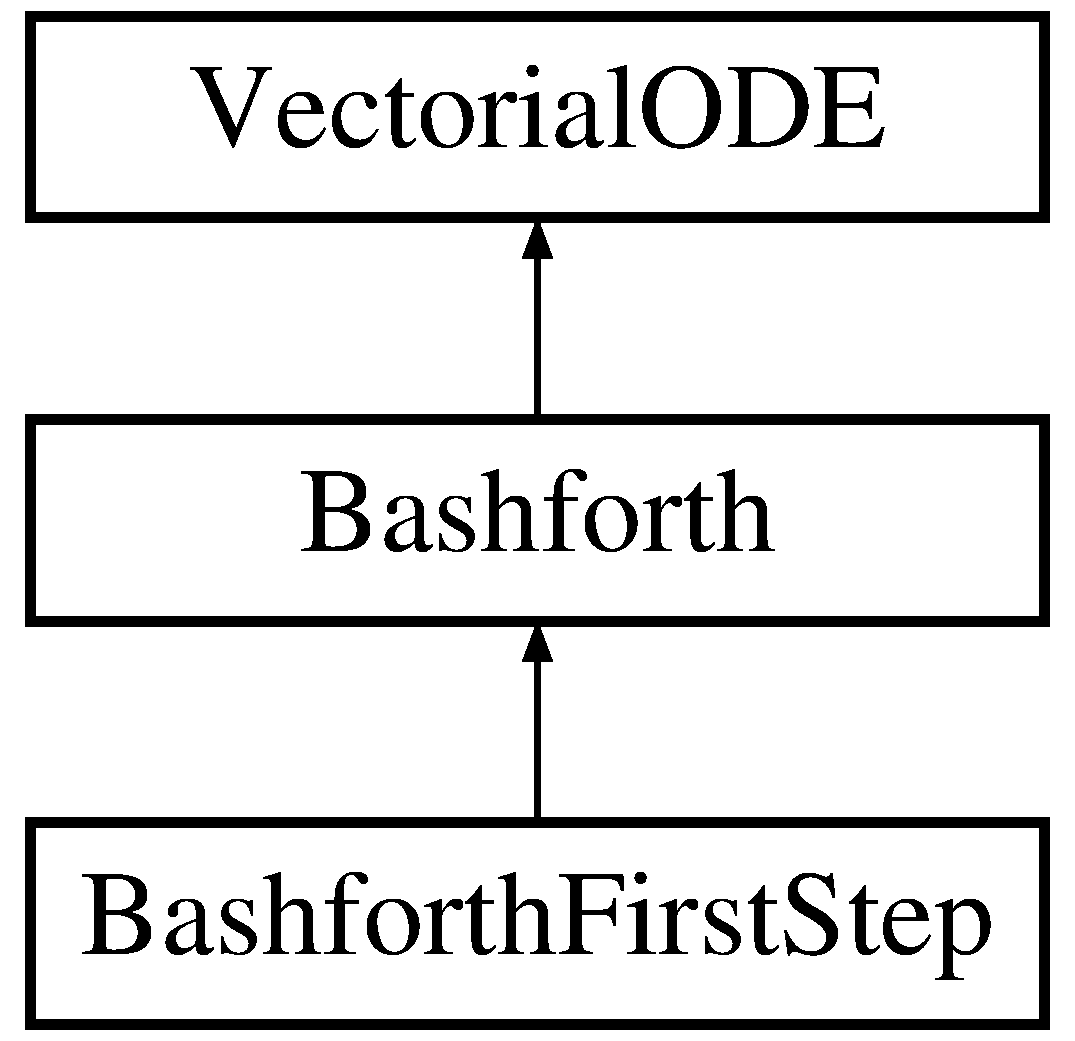
\includegraphics[height=3.000000cm]{class_bashforth_first_step}
\end{center}
\end{figure}
\subsection*{Public Member Functions}
\begin{DoxyCompactItemize}
\item 
\textbf{ Bashforth\+First\+Step} (\textbf{ Input} \&input, \textbf{ Solution} \&solution)
\begin{DoxyCompactList}\small\item\em Constructor inherited from the \doxyref{Bashforth}{p.}{class_bashforth} class (also inherited from \doxyref{Vectorial\+O\+DE}{p.}{class_vectorial_o_d_e}) \end{DoxyCompactList}\item 
void \textbf{ Solve\+Vectorial\+O\+DE} () override
\begin{DoxyCompactList}\small\item\em Method allowing the implementation of Adam-\/\+Bashforth method 1 step. This method is one of the several definition of the virtual inherited method. There are no arguments as all information needed are stored and are accessible in the input object. \end{DoxyCompactList}\end{DoxyCompactItemize}
\subsection*{Additional Inherited Members}


\subsection{Detailed Description}
Class implementing the Adam-\/\+Bashforth 1 step (Forward Euler) to solve the O\+DE system. \doxyref{Bashforth}{p.}{class_bashforth} method allows the solving of the O\+DE system. This class is implementing in such a way that it only writes the solution every Write\+Output\+Timestep. This class is inherited from \doxyref{Bashforth}{p.}{class_bashforth} class also inherited from \doxyref{Vectorial\+O\+DE}{p.}{class_vectorial_o_d_e}. 

\subsection{Constructor \& Destructor Documentation}
\mbox{\label{class_bashforth_first_step_a9bf484d3698f81dbd48665c78084f33e}} 
\index{Bashforth\+First\+Step@{Bashforth\+First\+Step}!Bashforth\+First\+Step@{Bashforth\+First\+Step}}
\index{Bashforth\+First\+Step@{Bashforth\+First\+Step}!Bashforth\+First\+Step@{Bashforth\+First\+Step}}
\subsubsection{Bashforth\+First\+Step()}
{\footnotesize\ttfamily Bashforth\+First\+Step\+::\+Bashforth\+First\+Step (\begin{DoxyParamCaption}\item[{\textbf{ Input} \&}]{input,  }\item[{\textbf{ Solution} \&}]{solution }\end{DoxyParamCaption})}



Constructor inherited from the \doxyref{Bashforth}{p.}{class_bashforth} class (also inherited from \doxyref{Vectorial\+O\+DE}{p.}{class_vectorial_o_d_e}) 


\begin{DoxyParams}{Parameters}
{\em input} & \+: \doxyref{Input}{p.}{class_input} object containing all variables needed to solve the O\+DE. \\
\hline
{\em solution} & \+: Output object where we will store the solution. \\
\hline
\end{DoxyParams}


\subsection{Member Function Documentation}
\mbox{\label{class_bashforth_first_step_a7d8f61b899c95a4339a8bdcf94124ea0}} 
\index{Bashforth\+First\+Step@{Bashforth\+First\+Step}!Solve\+Vectorial\+O\+DE@{Solve\+Vectorial\+O\+DE}}
\index{Solve\+Vectorial\+O\+DE@{Solve\+Vectorial\+O\+DE}!Bashforth\+First\+Step@{Bashforth\+First\+Step}}
\subsubsection{Solve\+Vectorial\+O\+D\+E()}
{\footnotesize\ttfamily void Bashforth\+First\+Step\+::\+Solve\+Vectorial\+O\+DE (\begin{DoxyParamCaption}{ }\end{DoxyParamCaption})\hspace{0.3cm}{\ttfamily [override]}, {\ttfamily [virtual]}}



Method allowing the implementation of Adam-\/\+Bashforth method 1 step. This method is one of the several definition of the virtual inherited method. There are no arguments as all information needed are stored and are accessible in the input object. 

\begin{DoxyReturn}{Returns}
Void return as the solution is stored in the solution object. 
\end{DoxyReturn}


Implements \textbf{ Bashforth} \doxyref{}{p.}{class_bashforth}.



The documentation for this class was generated from the following files\+:\begin{DoxyCompactItemize}
\item 
Bashforth\+First\+Step.\+h\item 
Bashforth\+First\+Step.\+cpp\end{DoxyCompactItemize}

\section{Bashforth\+Fourth\+Step Class Reference}
\label{class_bashforth_fourth_step}\index{Bashforth\+Fourth\+Step@{Bashforth\+Fourth\+Step}}


Class implementing the Adam-\/\+Bashforth 4 steps to solve the O\+DE system. \doxyref{Bashforth}{p.}{class_bashforth} method allows the solving of the O\+DE system. This class is implementing in such a way that it only writes the solution every Write\+Output\+Timestep. This class is inherited from \doxyref{Bashforth}{p.}{class_bashforth} class also inherited from \doxyref{Vectorial\+O\+DE}{p.}{class_vectorial_o_d_e}.  




{\ttfamily \#include $<$Bashforth\+Fourth\+Step.\+h$>$}

Inheritance diagram for Bashforth\+Fourth\+Step\+:\begin{figure}[H]
\begin{center}
\leavevmode
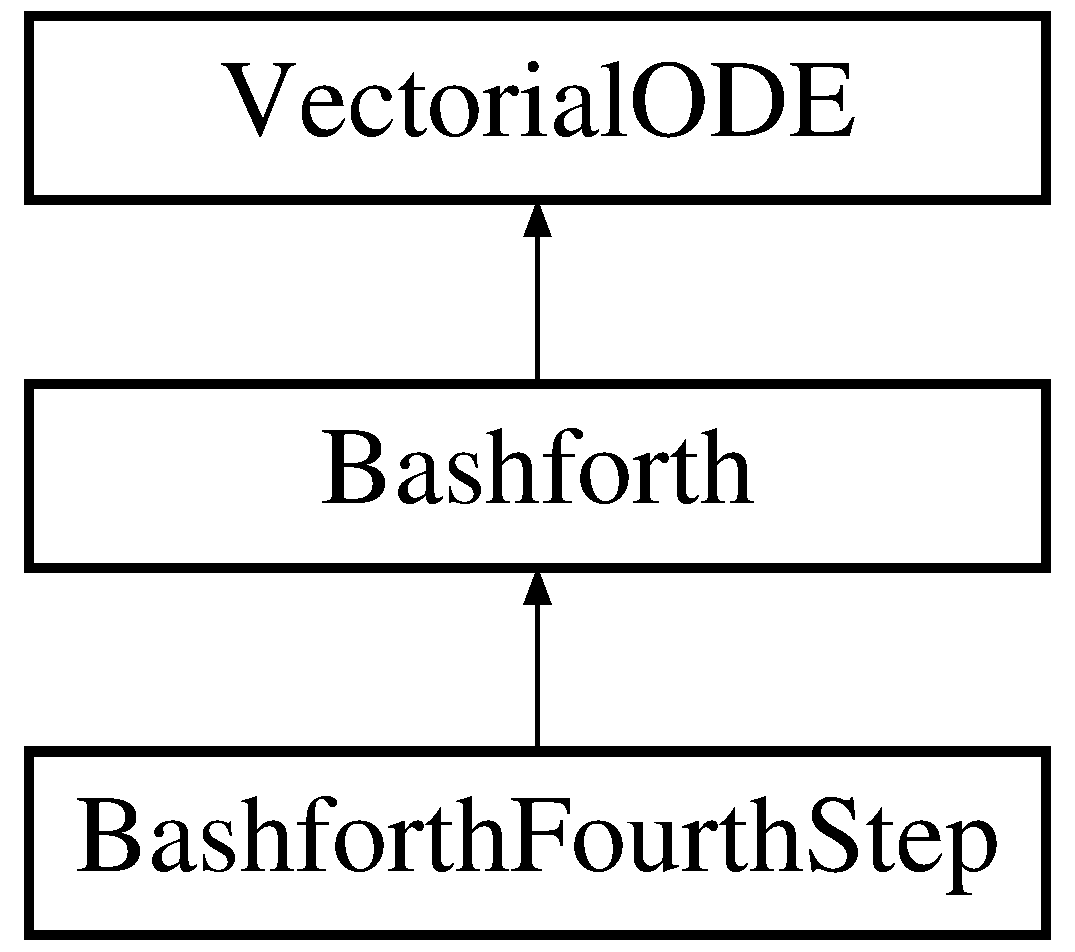
\includegraphics[height=3.000000cm]{class_bashforth_fourth_step}
\end{center}
\end{figure}
\subsection*{Public Member Functions}
\begin{DoxyCompactItemize}
\item 
\textbf{ Bashforth\+Fourth\+Step} (\textbf{ Input} \&input, \textbf{ Solution} \&solution)
\begin{DoxyCompactList}\small\item\em Constructor inherited from the \doxyref{Bashforth}{p.}{class_bashforth} class (also inherited from \doxyref{Vectorial\+O\+DE}{p.}{class_vectorial_o_d_e}) \end{DoxyCompactList}\item 
void \textbf{ Solve\+Vectorial\+O\+DE} () override
\begin{DoxyCompactList}\small\item\em Method allowing the implementation of Adam-\/\+Bashforth method 4 steps. This method is one of the several definition of the virtual inherited method. There are no arguments as all information needed are stored and are accessible in the input object. \end{DoxyCompactList}\end{DoxyCompactItemize}
\subsection*{Additional Inherited Members}


\subsection{Detailed Description}
Class implementing the Adam-\/\+Bashforth 4 steps to solve the O\+DE system. \doxyref{Bashforth}{p.}{class_bashforth} method allows the solving of the O\+DE system. This class is implementing in such a way that it only writes the solution every Write\+Output\+Timestep. This class is inherited from \doxyref{Bashforth}{p.}{class_bashforth} class also inherited from \doxyref{Vectorial\+O\+DE}{p.}{class_vectorial_o_d_e}. 

\subsection{Constructor \& Destructor Documentation}
\mbox{\label{class_bashforth_fourth_step_a0fb06f58a9a3863fb11102d5a7ef1a35}} 
\index{Bashforth\+Fourth\+Step@{Bashforth\+Fourth\+Step}!Bashforth\+Fourth\+Step@{Bashforth\+Fourth\+Step}}
\index{Bashforth\+Fourth\+Step@{Bashforth\+Fourth\+Step}!Bashforth\+Fourth\+Step@{Bashforth\+Fourth\+Step}}
\subsubsection{Bashforth\+Fourth\+Step()}
{\footnotesize\ttfamily Bashforth\+Fourth\+Step\+::\+Bashforth\+Fourth\+Step (\begin{DoxyParamCaption}\item[{\textbf{ Input} \&}]{input,  }\item[{\textbf{ Solution} \&}]{solution }\end{DoxyParamCaption})}



Constructor inherited from the \doxyref{Bashforth}{p.}{class_bashforth} class (also inherited from \doxyref{Vectorial\+O\+DE}{p.}{class_vectorial_o_d_e}) 


\begin{DoxyParams}{Parameters}
{\em input} & \+: \doxyref{Input}{p.}{class_input} object containing all variables needed to solve the O\+DE. \\
\hline
{\em solution} & \+: Output object where we will store the solution. \\
\hline
\end{DoxyParams}


\subsection{Member Function Documentation}
\mbox{\label{class_bashforth_fourth_step_a0939c51b0c500627728eaee93f5d0d5c}} 
\index{Bashforth\+Fourth\+Step@{Bashforth\+Fourth\+Step}!Solve\+Vectorial\+O\+DE@{Solve\+Vectorial\+O\+DE}}
\index{Solve\+Vectorial\+O\+DE@{Solve\+Vectorial\+O\+DE}!Bashforth\+Fourth\+Step@{Bashforth\+Fourth\+Step}}
\subsubsection{Solve\+Vectorial\+O\+D\+E()}
{\footnotesize\ttfamily void Bashforth\+Fourth\+Step\+::\+Solve\+Vectorial\+O\+DE (\begin{DoxyParamCaption}{ }\end{DoxyParamCaption})\hspace{0.3cm}{\ttfamily [override]}, {\ttfamily [virtual]}}



Method allowing the implementation of Adam-\/\+Bashforth method 4 steps. This method is one of the several definition of the virtual inherited method. There are no arguments as all information needed are stored and are accessible in the input object. 

\begin{DoxyReturn}{Returns}
Void return as the solution is stored in the solution object. 
\end{DoxyReturn}


Implements \textbf{ Bashforth} \doxyref{}{p.}{class_bashforth}.



The documentation for this class was generated from the following files\+:\begin{DoxyCompactItemize}
\item 
Bashforth\+Fourth\+Step.\+h\item 
Bashforth\+Fourth\+Step.\+cpp\end{DoxyCompactItemize}

\section{Bashforth\+Second\+Step Class Reference}
\label{class_bashforth_second_step}\index{Bashforth\+Second\+Step@{Bashforth\+Second\+Step}}


Class implementing the Adam-\/\+Bashforth 2 steps to solve the O\+DE system. \doxyref{Bashforth}{p.}{class_bashforth} method allows the solving of the O\+DE system. This class is implementing in such a way that it only writes the solution every Write\+Output\+Timestep. This class is inherited from \doxyref{Bashforth}{p.}{class_bashforth} class also inherited from \doxyref{Vectorial\+O\+DE}{p.}{class_vectorial_o_d_e}.  




{\ttfamily \#include $<$Bashforth\+Second\+Step.\+h$>$}

Inheritance diagram for Bashforth\+Second\+Step\+:\begin{figure}[H]
\begin{center}
\leavevmode
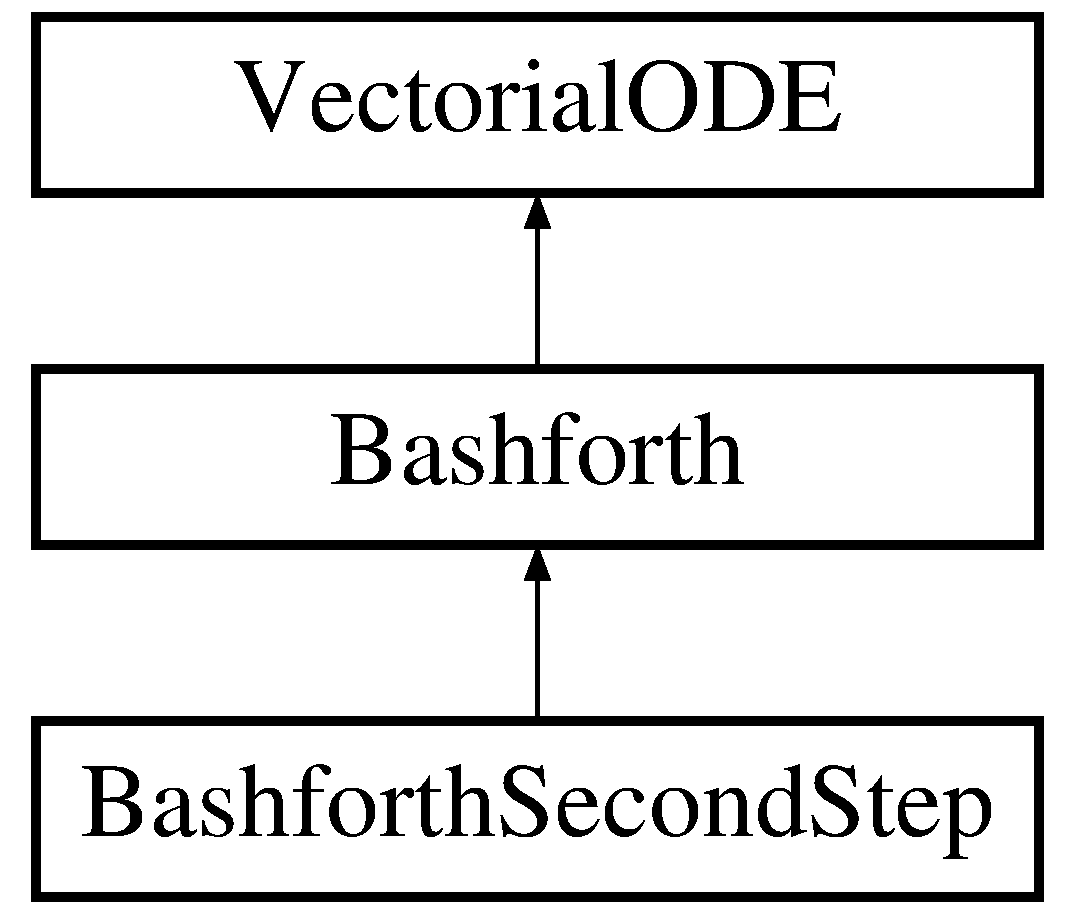
\includegraphics[height=3.000000cm]{class_bashforth_second_step}
\end{center}
\end{figure}
\subsection*{Public Member Functions}
\begin{DoxyCompactItemize}
\item 
\textbf{ Bashforth\+Second\+Step} (\textbf{ Input} \&input, \textbf{ Solution} \&solution)
\begin{DoxyCompactList}\small\item\em \+: Constructor inherited from the \doxyref{Bashforth}{p.}{class_bashforth} class (also inherited from \doxyref{Vectorial\+O\+DE}{p.}{class_vectorial_o_d_e}) \end{DoxyCompactList}\item 
void \textbf{ Solve\+Vectorial\+O\+DE} () override
\begin{DoxyCompactList}\small\item\em Method allowing the implementation of Adam-\/\+Bashforth method 2 steps. This method is one of the several definition of the virtual inherited method. There are no arguments as all information needed are stored and are accessible in the input object. \end{DoxyCompactList}\end{DoxyCompactItemize}
\subsection*{Additional Inherited Members}


\subsection{Detailed Description}
Class implementing the Adam-\/\+Bashforth 2 steps to solve the O\+DE system. \doxyref{Bashforth}{p.}{class_bashforth} method allows the solving of the O\+DE system. This class is implementing in such a way that it only writes the solution every Write\+Output\+Timestep. This class is inherited from \doxyref{Bashforth}{p.}{class_bashforth} class also inherited from \doxyref{Vectorial\+O\+DE}{p.}{class_vectorial_o_d_e}. 

\subsection{Constructor \& Destructor Documentation}
\mbox{\label{class_bashforth_second_step_a4cdea92719d28a26543d78792d8b6ed1}} 
\index{Bashforth\+Second\+Step@{Bashforth\+Second\+Step}!Bashforth\+Second\+Step@{Bashforth\+Second\+Step}}
\index{Bashforth\+Second\+Step@{Bashforth\+Second\+Step}!Bashforth\+Second\+Step@{Bashforth\+Second\+Step}}
\subsubsection{Bashforth\+Second\+Step()}
{\footnotesize\ttfamily Bashforth\+Second\+Step\+::\+Bashforth\+Second\+Step (\begin{DoxyParamCaption}\item[{\textbf{ Input} \&}]{input,  }\item[{\textbf{ Solution} \&}]{solution }\end{DoxyParamCaption})}



\+: Constructor inherited from the \doxyref{Bashforth}{p.}{class_bashforth} class (also inherited from \doxyref{Vectorial\+O\+DE}{p.}{class_vectorial_o_d_e}) 


\begin{DoxyParams}{Parameters}
{\em input} & \+: \doxyref{Input}{p.}{class_input} object containing all variables needed to solve the O\+DE. \\
\hline
{\em solution} & \+: Output object where we will store the solution. \\
\hline
\end{DoxyParams}


\subsection{Member Function Documentation}
\mbox{\label{class_bashforth_second_step_af2470291d9aa30f4d106b92fc08bda88}} 
\index{Bashforth\+Second\+Step@{Bashforth\+Second\+Step}!Solve\+Vectorial\+O\+DE@{Solve\+Vectorial\+O\+DE}}
\index{Solve\+Vectorial\+O\+DE@{Solve\+Vectorial\+O\+DE}!Bashforth\+Second\+Step@{Bashforth\+Second\+Step}}
\subsubsection{Solve\+Vectorial\+O\+D\+E()}
{\footnotesize\ttfamily void Bashforth\+Second\+Step\+::\+Solve\+Vectorial\+O\+DE (\begin{DoxyParamCaption}{ }\end{DoxyParamCaption})\hspace{0.3cm}{\ttfamily [override]}, {\ttfamily [virtual]}}



Method allowing the implementation of Adam-\/\+Bashforth method 2 steps. This method is one of the several definition of the virtual inherited method. There are no arguments as all information needed are stored and are accessible in the input object. 

\begin{DoxyReturn}{Returns}
Void return as the solution is stored in the solution object. 
\end{DoxyReturn}


Implements \textbf{ Bashforth} \doxyref{}{p.}{class_bashforth}.



The documentation for this class was generated from the following files\+:\begin{DoxyCompactItemize}
\item 
Bashforth\+Second\+Step.\+h\item 
Bashforth\+Second\+Step.\+cpp\end{DoxyCompactItemize}

\section{Bashforth\+Third\+Step Class Reference}
\label{class_bashforth_third_step}\index{Bashforth\+Third\+Step@{Bashforth\+Third\+Step}}


Class implementing the Adam-\/\+Bashforth 3 steps to solve the O\+DE system. \doxyref{Bashforth}{p.}{class_bashforth} method allows the solving of the O\+DE system. This class is implementing in such a way that it only writes the solution every Write\+Output\+Timestep. This class is inherited from \doxyref{Bashforth}{p.}{class_bashforth} class also inherited from \doxyref{Vectorial\+O\+DE}{p.}{class_vectorial_o_d_e}.  




{\ttfamily \#include $<$Bashforth\+Third\+Step.\+h$>$}

Inheritance diagram for Bashforth\+Third\+Step\+:\begin{figure}[H]
\begin{center}
\leavevmode
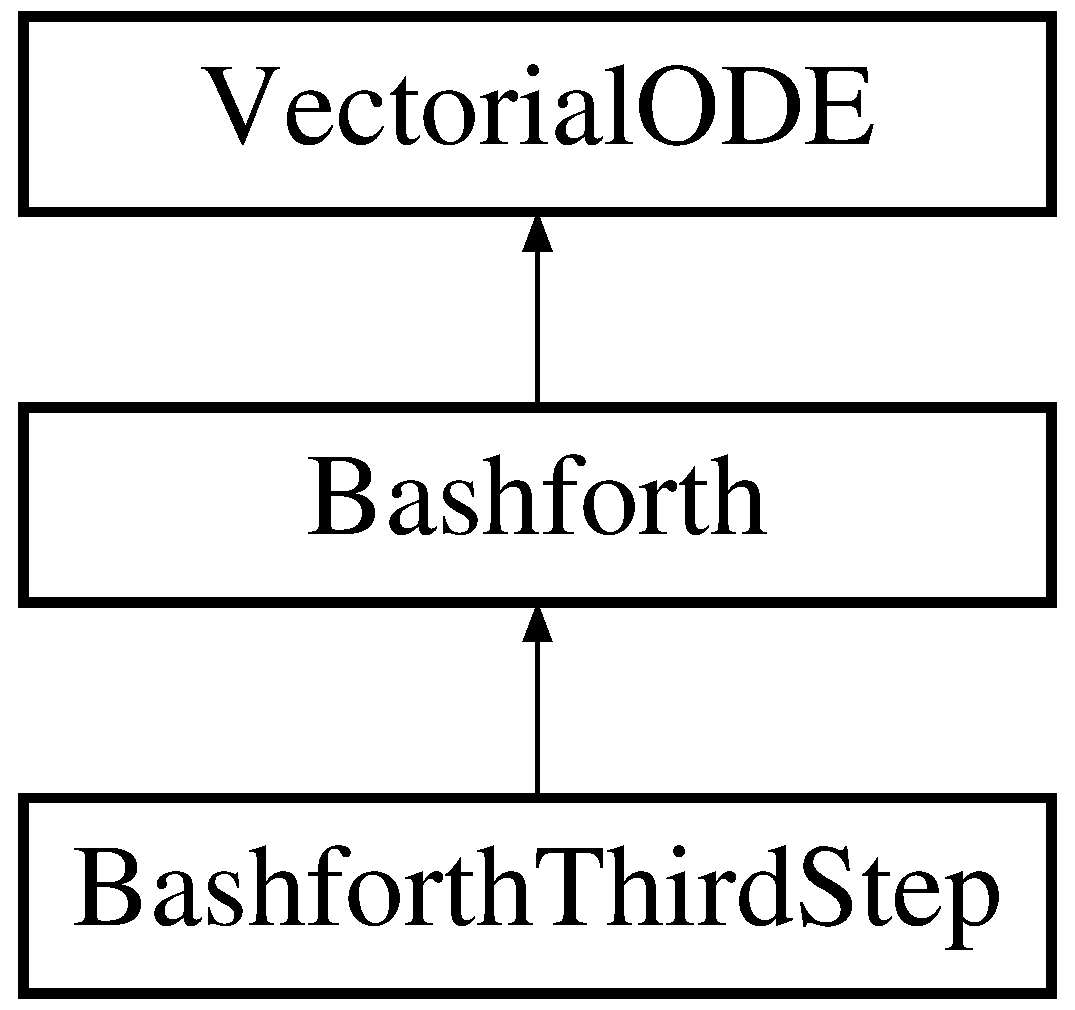
\includegraphics[height=3.000000cm]{class_bashforth_third_step}
\end{center}
\end{figure}
\subsection*{Public Member Functions}
\begin{DoxyCompactItemize}
\item 
\textbf{ Bashforth\+Third\+Step} (\textbf{ Input} \&input, \textbf{ Solution} \&solution)
\begin{DoxyCompactList}\small\item\em Constructor inherited from the \doxyref{Bashforth}{p.}{class_bashforth} class (also inherited from \doxyref{Vectorial\+O\+DE}{p.}{class_vectorial_o_d_e}) \end{DoxyCompactList}\item 
void \textbf{ Solve\+Vectorial\+O\+DE} () override
\begin{DoxyCompactList}\small\item\em Method allowing the implementation of Adam-\/\+Bashforth method 3 steps. This method is one of the several definition of the virtual inherited method. There are no arguments as all information needed are stored and are accessible in the input object. \end{DoxyCompactList}\end{DoxyCompactItemize}
\subsection*{Additional Inherited Members}


\subsection{Detailed Description}
Class implementing the Adam-\/\+Bashforth 3 steps to solve the O\+DE system. \doxyref{Bashforth}{p.}{class_bashforth} method allows the solving of the O\+DE system. This class is implementing in such a way that it only writes the solution every Write\+Output\+Timestep. This class is inherited from \doxyref{Bashforth}{p.}{class_bashforth} class also inherited from \doxyref{Vectorial\+O\+DE}{p.}{class_vectorial_o_d_e}. 

\subsection{Constructor \& Destructor Documentation}
\mbox{\label{class_bashforth_third_step_ae7c2a0560bae50933836e2b975402fdd}} 
\index{Bashforth\+Third\+Step@{Bashforth\+Third\+Step}!Bashforth\+Third\+Step@{Bashforth\+Third\+Step}}
\index{Bashforth\+Third\+Step@{Bashforth\+Third\+Step}!Bashforth\+Third\+Step@{Bashforth\+Third\+Step}}
\subsubsection{Bashforth\+Third\+Step()}
{\footnotesize\ttfamily Bashforth\+Third\+Step\+::\+Bashforth\+Third\+Step (\begin{DoxyParamCaption}\item[{\textbf{ Input} \&}]{input,  }\item[{\textbf{ Solution} \&}]{solution }\end{DoxyParamCaption})}



Constructor inherited from the \doxyref{Bashforth}{p.}{class_bashforth} class (also inherited from \doxyref{Vectorial\+O\+DE}{p.}{class_vectorial_o_d_e}) 


\begin{DoxyParams}{Parameters}
{\em input} & \+: \doxyref{Input}{p.}{class_input} object containing all variables needed to solve the O\+DE. \\
\hline
{\em solution} & \+: Output object where we will store the solution. \\
\hline
\end{DoxyParams}


\subsection{Member Function Documentation}
\mbox{\label{class_bashforth_third_step_ae20b385fcae5a61ebee617250577a40a}} 
\index{Bashforth\+Third\+Step@{Bashforth\+Third\+Step}!Solve\+Vectorial\+O\+DE@{Solve\+Vectorial\+O\+DE}}
\index{Solve\+Vectorial\+O\+DE@{Solve\+Vectorial\+O\+DE}!Bashforth\+Third\+Step@{Bashforth\+Third\+Step}}
\subsubsection{Solve\+Vectorial\+O\+D\+E()}
{\footnotesize\ttfamily void Bashforth\+Third\+Step\+::\+Solve\+Vectorial\+O\+DE (\begin{DoxyParamCaption}{ }\end{DoxyParamCaption})\hspace{0.3cm}{\ttfamily [override]}, {\ttfamily [virtual]}}



Method allowing the implementation of Adam-\/\+Bashforth method 3 steps. This method is one of the several definition of the virtual inherited method. There are no arguments as all information needed are stored and are accessible in the input object. 

\begin{DoxyReturn}{Returns}
Void return as the solution is stored in the solution object. 
\end{DoxyReturn}


Implements \textbf{ Bashforth} \doxyref{}{p.}{class_bashforth}.



The documentation for this class was generated from the following files\+:\begin{DoxyCompactItemize}
\item 
Bashforth\+Third\+Step.\+h\item 
Bashforth\+Third\+Step.\+cpp\end{DoxyCompactItemize}

\section{Input Class Reference}
\label{class_input}\index{Input@{Input}}


Class allowing the saving of all the variables to define the system we want to solve. In fact, it takes as input variable (integer or double)\+: Timestep, Dimension, Order, Number\+Steps, Write\+Output\+Timestep. Moreover, \doxyref{Input}{p.}{class_input} object needs 3 matrix to define the system \+: Initial\+Condition\+Matrix, Coefficient\+Matrix, Function\+Matrix. Matrix are defined to be vector of vector of double. \doxyref{Input}{p.}{class_input} variables are given to the input class by the constructor. The other methods are getter allowing the access to theses private attributes.  




{\ttfamily \#include $<$Input.\+h$>$}

\subsection*{Public Member Functions}
\begin{DoxyCompactItemize}
\item 
\mbox{\label{class_input_abae3f379d3f157cf42dc857309832dba}} 
\textbf{ Input} ()
\begin{DoxyCompactList}\small\item\em Constructor allowing the definition of the system we want to solve. In this class, the three input matrix were hardcode with the order of the system. \end{DoxyCompactList}\item 
\textbf{ Input} (double time\+\_\+step, int dimension, int order, int number\+\_\+steps, int write\+\_\+output\+\_\+timestep, const vector$<$ vector$<$ double $>$$>$ \&initial\+\_\+condition\+\_\+matrix, const vector$<$ vector$<$ double $>$$>$ \&changing\+\_\+matrix, const vector$<$ vector$<$ double $>$$>$ \&past\+\_\+step\+\_\+matrix)
\begin{DoxyCompactList}\small\item\em Constructor of the class allowing the definition of the system. \end{DoxyCompactList}\item 
int \textbf{ Ask\+Number\+To\+User} ()
\begin{DoxyCompactList}\small\item\em Method allowing the asking of a number to the user. The user will enter this input number thank to the keyboard. \end{DoxyCompactList}\item 
\mbox{\label{class_input_a47ccd0138fd87abb7ddbaae502930c45}} 
double \& \textbf{ Get\+Timestep} () const
\begin{DoxyCompactList}\small\item\em Return the time step attribute. \end{DoxyCompactList}\item 
\mbox{\label{class_input_a1fff5b534cc24e5ac8651366fa9cc8c1}} 
unsigned long \textbf{ Get\+Dimension} () const
\begin{DoxyCompactList}\small\item\em Return the dimension attribute. \end{DoxyCompactList}\item 
\mbox{\label{class_input_ab4191112b8950f47f14a4407816b07d5}} 
int \& \textbf{ Get\+Order} () const
\begin{DoxyCompactList}\small\item\em Return the solver attribute. \end{DoxyCompactList}\item 
\mbox{\label{class_input_aef65eb3f06d64b552f38d57935cb5352}} 
int \& \textbf{ Get\+Number\+Steps} () const
\begin{DoxyCompactList}\small\item\em Return the overall number of steps attribute. \end{DoxyCompactList}\item 
\mbox{\label{class_input_ae42ae51a450a823789f86b02bfbbcb0e}} 
int \& \textbf{ Get\+Write\+Output\+Timestep} () const
\begin{DoxyCompactList}\small\item\em Return the Timestep defining when we write the output solution. \end{DoxyCompactList}\item 
\mbox{\label{class_input_a13947607d3f8e48c5d4db22d729f2674}} 
vector$<$ vector$<$ double $>$ $>$ \textbf{ Get\+Initial\+Condition\+Matrix} () const
\begin{DoxyCompactList}\small\item\em Return the initial condition matrix. \end{DoxyCompactList}\item 
\mbox{\label{class_input_ad4cbcaa4be06227c960cf30629af44ea}} 
vector$<$ vector$<$ double $>$ $>$ \textbf{ Get\+Coefficient\+Matrix} () const
\begin{DoxyCompactList}\small\item\em Return the changing matrix corresponding to several states when the program run. \end{DoxyCompactList}\item 
\mbox{\label{class_input_ab1813f72891b82c461ab2a075fbd8d00}} 
vector$<$ vector$<$ double $>$ $>$ \textbf{ Get\+Function\+Matrix} () const
\begin{DoxyCompactList}\small\item\em Return the past step corresponding to i-\/1 for the function defining the problem. \end{DoxyCompactList}\item 
\mbox{\label{class_input_af2db35ba67c8a8ccd23bef6a482fc291}} 
\textbf{ $\sim$\+Input} ()
\begin{DoxyCompactList}\small\item\em Destructor allowing the liberation of memory. \end{DoxyCompactList}\end{DoxyCompactItemize}


\subsection{Detailed Description}
Class allowing the saving of all the variables to define the system we want to solve. In fact, it takes as input variable (integer or double)\+: Timestep, Dimension, Order, Number\+Steps, Write\+Output\+Timestep. Moreover, \doxyref{Input}{p.}{class_input} object needs 3 matrix to define the system \+: Initial\+Condition\+Matrix, Coefficient\+Matrix, Function\+Matrix. Matrix are defined to be vector of vector of double. \doxyref{Input}{p.}{class_input} variables are given to the input class by the constructor. The other methods are getter allowing the access to theses private attributes. 

\subsection{Constructor \& Destructor Documentation}
\mbox{\label{class_input_a6e9028a0843a2db4271a4e3bf3eb941f}} 
\index{Input@{Input}!Input@{Input}}
\index{Input@{Input}!Input@{Input}}
\subsubsection{Input()}
{\footnotesize\ttfamily Input\+::\+Input (\begin{DoxyParamCaption}\item[{double}]{time\+\_\+step,  }\item[{int}]{dimension,  }\item[{int}]{order,  }\item[{int}]{number\+\_\+steps,  }\item[{int}]{write\+\_\+output\+\_\+timestep,  }\item[{const vector$<$ vector$<$ double $>$$>$ \&}]{initial\+\_\+condition\+\_\+matrix,  }\item[{const vector$<$ vector$<$ double $>$$>$ \&}]{coefficient\+\_\+matrix,  }\item[{const vector$<$ vector$<$ double $>$$>$ \&}]{function\+\_\+matrix }\end{DoxyParamCaption})\hspace{0.3cm}{\ttfamily [explicit]}}



Constructor of the class allowing the definition of the system. 


\begin{DoxyParams}{Parameters}
{\em time\+\_\+step} & \+: Double representing the time step we will use in the O\+DE solver. \\
\hline
{\em dimension} & \+: Integer representing the dimension of the system. \\
\hline
{\em order} & \+: Integer representing the order of the system. \\
\hline
{\em number\+\_\+steps} & \+: Integer representing the overall number of steps we will do to solve the system. \\
\hline
{\em write\+\_\+output\+\_\+timestep} & \+: Integer representing the steps when we write the solutions \\
\hline
{\em initial\+\_\+condition\+\_\+matrix} & \+: Matrix (which is a vector of vector of double) representing the initial conditions of the system. \\
\hline
{\em coefficient\+\_\+matrix} & \+: Matrix (which is a vector of vector of double) containing the value of the function defining the system for all the step we want to compute. \\
\hline
{\em function\+\_\+matrix} & \+: Matrix (which is a vector of vector of double) allowing the definition of the R\+HS of the O\+DE. \\
\hline
\end{DoxyParams}


\subsection{Member Function Documentation}
\mbox{\label{class_input_ae6eae7ea32488c4ce43a027b3b2fabc2}} 
\index{Input@{Input}!Ask\+Number\+To\+User@{Ask\+Number\+To\+User}}
\index{Ask\+Number\+To\+User@{Ask\+Number\+To\+User}!Input@{Input}}
\subsubsection{Ask\+Number\+To\+User()}
{\footnotesize\ttfamily int Input\+::\+Ask\+Number\+To\+User (\begin{DoxyParamCaption}{ }\end{DoxyParamCaption})}



Method allowing the asking of a number to the user. The user will enter this input number thank to the keyboard. 

\begin{DoxyReturn}{Returns}
\+: Returns the integer number given by the user. 
\end{DoxyReturn}


The documentation for this class was generated from the following files\+:\begin{DoxyCompactItemize}
\item 
Input.\+h\item 
Input.\+cpp\end{DoxyCompactItemize}

\section{Runge\+Kutta Class Reference}
\label{class_runge_kutta}\index{Runge\+Kutta@{Runge\+Kutta}}


Class allowing a more precise definition of one of the O\+DE solvers technics which is Runge-\/\+Kutta method. This is an abstract class as before because the method Solve\+Vectorial\+O\+DE is virtual and it will be defined in different ways in the inherited classes. The different Runge-\/\+Kutta method correspond to the different order we use to solve the system.  




{\ttfamily \#include $<$Runge\+Kutta.\+h$>$}

Inheritance diagram for Runge\+Kutta\+:\begin{figure}[H]
\begin{center}
\leavevmode
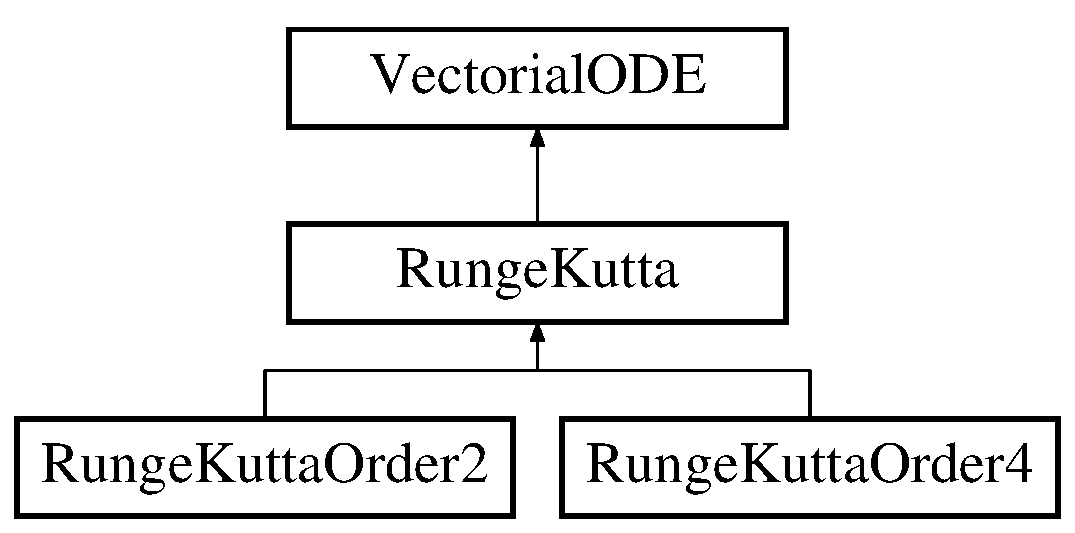
\includegraphics[height=3.000000cm]{class_runge_kutta}
\end{center}
\end{figure}
\subsection*{Public Member Functions}
\begin{DoxyCompactItemize}
\item 
\textbf{ Runge\+Kutta} (\textbf{ Input} \&input, \textbf{ Solution} \&solution)
\begin{DoxyCompactList}\small\item\em Constructor inherited from the \doxyref{Vectorial\+O\+DE}{p.}{class_vectorial_o_d_e} class. \end{DoxyCompactList}\item 
\mbox{\label{class_runge_kutta_a6282be932f2dc501deb099f071953ae2}} 
virtual void {\bfseries Solve\+Vectorial\+O\+DE} ()=0
\end{DoxyCompactItemize}
\subsection*{Additional Inherited Members}


\subsection{Detailed Description}
Class allowing a more precise definition of one of the O\+DE solvers technics which is Runge-\/\+Kutta method. This is an abstract class as before because the method Solve\+Vectorial\+O\+DE is virtual and it will be defined in different ways in the inherited classes. The different Runge-\/\+Kutta method correspond to the different order we use to solve the system. 

\subsection{Constructor \& Destructor Documentation}
\mbox{\label{class_runge_kutta_a578f5ec321d4228db31b2dd21091c3da}} 
\index{Runge\+Kutta@{Runge\+Kutta}!Runge\+Kutta@{Runge\+Kutta}}
\index{Runge\+Kutta@{Runge\+Kutta}!Runge\+Kutta@{Runge\+Kutta}}
\subsubsection{Runge\+Kutta()}
{\footnotesize\ttfamily Runge\+Kutta\+::\+Runge\+Kutta (\begin{DoxyParamCaption}\item[{\textbf{ Input} \&}]{input,  }\item[{\textbf{ Solution} \&}]{solution }\end{DoxyParamCaption})}



Constructor inherited from the \doxyref{Vectorial\+O\+DE}{p.}{class_vectorial_o_d_e} class. 


\begin{DoxyParams}{Parameters}
{\em input} & \+: \doxyref{Input}{p.}{class_input} object containing all variables needed to solve the O\+DE. \\
\hline
{\em solution} & \+: Output object where we will store the solution. \\
\hline
\end{DoxyParams}


The documentation for this class was generated from the following files\+:\begin{DoxyCompactItemize}
\item 
Runge\+Kutta.\+h\item 
Runge\+Kutta.\+cpp\end{DoxyCompactItemize}

\section{Runge\+Kutta\+Order2 Class Reference}
\label{class_runge_kutta_order2}\index{Runge\+Kutta\+Order2@{Runge\+Kutta\+Order2}}


Class implementing the Runge-\/\+Kutta 2 steps to solve the O\+DE system. Runge-\/\+Kutta method allows the solving of the O\+DE system. This class is implementing in such a way that it only writes the solution every Write\+Output\+Timestep. This class is inherited from \doxyref{Runge\+Kutta}{p.}{class_runge_kutta} class also inherited from \doxyref{Vectorial\+O\+DE}{p.}{class_vectorial_o_d_e}.  




{\ttfamily \#include $<$Runge\+Kutta\+Order2.\+h$>$}

Inheritance diagram for Runge\+Kutta\+Order2\+:\begin{figure}[H]
\begin{center}
\leavevmode
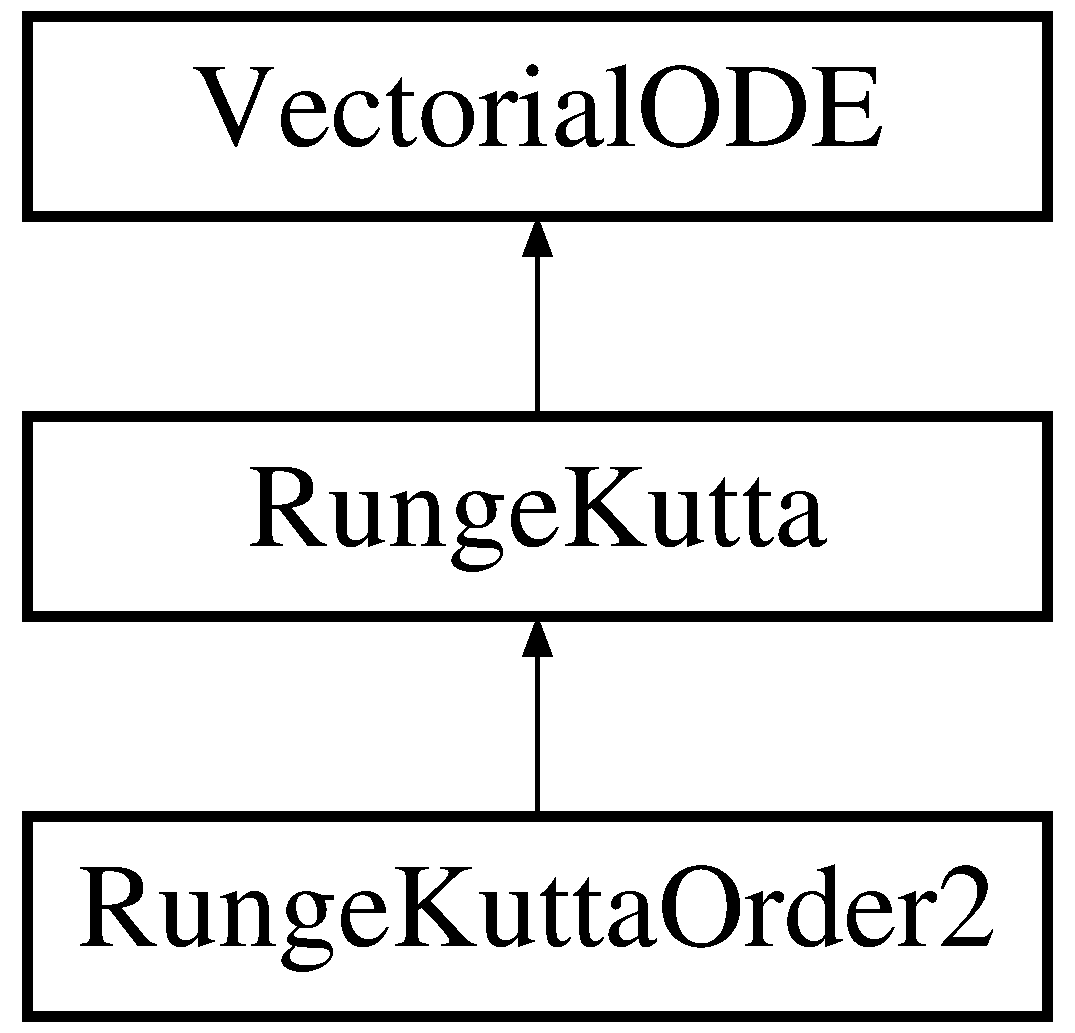
\includegraphics[height=3.000000cm]{class_runge_kutta_order2}
\end{center}
\end{figure}
\subsection*{Public Member Functions}
\begin{DoxyCompactItemize}
\item 
\textbf{ Runge\+Kutta\+Order2} (\textbf{ Input} \&input, \textbf{ Solution} \&solution)
\begin{DoxyCompactList}\small\item\em Constructor inherited from the \doxyref{Runge\+Kutta}{p.}{class_runge_kutta} class (also inherited from \doxyref{Vectorial\+O\+DE}{p.}{class_vectorial_o_d_e}) \end{DoxyCompactList}\item 
void \textbf{ Solve\+Vectorial\+O\+DE} () override
\begin{DoxyCompactList}\small\item\em Method allowing the implementation of Runge-\/\+Kutta method 2 step. This method is one of the several definition of the virtual inherited method. There are no arguments as all information needed are stored and are accessible in the input object. \end{DoxyCompactList}\end{DoxyCompactItemize}
\subsection*{Additional Inherited Members}


\subsection{Detailed Description}
Class implementing the Runge-\/\+Kutta 2 steps to solve the O\+DE system. Runge-\/\+Kutta method allows the solving of the O\+DE system. This class is implementing in such a way that it only writes the solution every Write\+Output\+Timestep. This class is inherited from \doxyref{Runge\+Kutta}{p.}{class_runge_kutta} class also inherited from \doxyref{Vectorial\+O\+DE}{p.}{class_vectorial_o_d_e}. 

\subsection{Constructor \& Destructor Documentation}
\mbox{\label{class_runge_kutta_order2_aa3a6b47fb671f0188a7150ab5a82a3c0}} 
\index{Runge\+Kutta\+Order2@{Runge\+Kutta\+Order2}!Runge\+Kutta\+Order2@{Runge\+Kutta\+Order2}}
\index{Runge\+Kutta\+Order2@{Runge\+Kutta\+Order2}!Runge\+Kutta\+Order2@{Runge\+Kutta\+Order2}}
\subsubsection{Runge\+Kutta\+Order2()}
{\footnotesize\ttfamily Runge\+Kutta\+Order2\+::\+Runge\+Kutta\+Order2 (\begin{DoxyParamCaption}\item[{\textbf{ Input} \&}]{input,  }\item[{\textbf{ Solution} \&}]{solution }\end{DoxyParamCaption})}



Constructor inherited from the \doxyref{Runge\+Kutta}{p.}{class_runge_kutta} class (also inherited from \doxyref{Vectorial\+O\+DE}{p.}{class_vectorial_o_d_e}) 


\begin{DoxyParams}{Parameters}
{\em input} & \+: \doxyref{Input}{p.}{class_input} object containing all variables needed to solve the O\+DE. \\
\hline
{\em solution} & \+: Output object where we will store the solution. \\
\hline
\end{DoxyParams}


\subsection{Member Function Documentation}
\mbox{\label{class_runge_kutta_order2_a87a676d85bac25f23c3cd5485b005a9f}} 
\index{Runge\+Kutta\+Order2@{Runge\+Kutta\+Order2}!Solve\+Vectorial\+O\+DE@{Solve\+Vectorial\+O\+DE}}
\index{Solve\+Vectorial\+O\+DE@{Solve\+Vectorial\+O\+DE}!Runge\+Kutta\+Order2@{Runge\+Kutta\+Order2}}
\subsubsection{Solve\+Vectorial\+O\+D\+E()}
{\footnotesize\ttfamily void Runge\+Kutta\+Order2\+::\+Solve\+Vectorial\+O\+DE (\begin{DoxyParamCaption}{ }\end{DoxyParamCaption})\hspace{0.3cm}{\ttfamily [override]}, {\ttfamily [virtual]}}



Method allowing the implementation of Runge-\/\+Kutta method 2 step. This method is one of the several definition of the virtual inherited method. There are no arguments as all information needed are stored and are accessible in the input object. 

\begin{DoxyReturn}{Returns}
Void return as the solution is stored in the solution object. 
\end{DoxyReturn}


Implements \textbf{ Runge\+Kutta} \doxyref{}{p.}{class_runge_kutta}.



The documentation for this class was generated from the following files\+:\begin{DoxyCompactItemize}
\item 
Runge\+Kutta\+Order2.\+h\item 
Runge\+Kutta\+Order2.\+cpp\end{DoxyCompactItemize}

\section{Runge\+Kutta\+Order4 Class Reference}
\label{class_runge_kutta_order4}\index{Runge\+Kutta\+Order4@{Runge\+Kutta\+Order4}}


Class implementing the Runge-\/\+Kutta 4 steps to solve the O\+DE system. Runge-\/\+Kutta method allows the solving of the O\+DE system. This class is implementing in such a way that it only writes the solution every Write\+Output\+Timestep. This class is inherited from \doxyref{Runge\+Kutta}{p.}{class_runge_kutta} class also inherited from \doxyref{Vectorial\+O\+DE}{p.}{class_vectorial_o_d_e}.  




{\ttfamily \#include $<$Runge\+Kutta\+Order4.\+h$>$}

Inheritance diagram for Runge\+Kutta\+Order4\+:\begin{figure}[H]
\begin{center}
\leavevmode
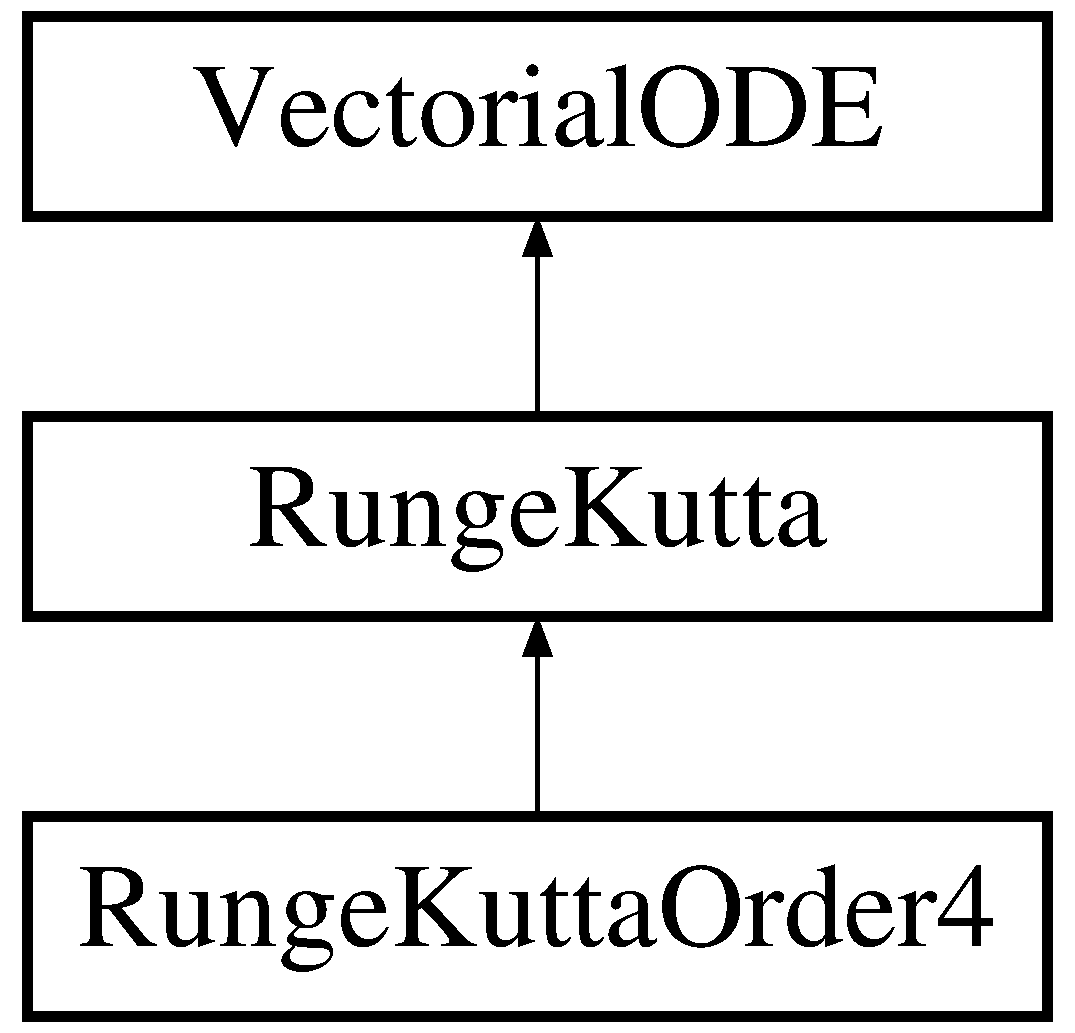
\includegraphics[height=3.000000cm]{class_runge_kutta_order4}
\end{center}
\end{figure}
\subsection*{Public Member Functions}
\begin{DoxyCompactItemize}
\item 
\textbf{ Runge\+Kutta\+Order4} (\textbf{ Input} \&input, \textbf{ Solution} \&solution)
\begin{DoxyCompactList}\small\item\em Constructor inherited from the \doxyref{Runge\+Kutta}{p.}{class_runge_kutta} class (also inherited from \doxyref{Vectorial\+O\+DE}{p.}{class_vectorial_o_d_e}) \end{DoxyCompactList}\item 
void \textbf{ Solve\+Vectorial\+O\+DE} () override
\begin{DoxyCompactList}\small\item\em Method allowing the implementation of Runge-\/\+Kutta method 4 step. This method is one of the several definition of the virtual inherited method. There are no arguments as all information needed are stored and are accessible in the input object. \end{DoxyCompactList}\end{DoxyCompactItemize}
\subsection*{Additional Inherited Members}


\subsection{Detailed Description}
Class implementing the Runge-\/\+Kutta 4 steps to solve the O\+DE system. Runge-\/\+Kutta method allows the solving of the O\+DE system. This class is implementing in such a way that it only writes the solution every Write\+Output\+Timestep. This class is inherited from \doxyref{Runge\+Kutta}{p.}{class_runge_kutta} class also inherited from \doxyref{Vectorial\+O\+DE}{p.}{class_vectorial_o_d_e}. 

\subsection{Constructor \& Destructor Documentation}
\mbox{\label{class_runge_kutta_order4_a599bea2c5f1f537f8874f6c354e36f44}} 
\index{Runge\+Kutta\+Order4@{Runge\+Kutta\+Order4}!Runge\+Kutta\+Order4@{Runge\+Kutta\+Order4}}
\index{Runge\+Kutta\+Order4@{Runge\+Kutta\+Order4}!Runge\+Kutta\+Order4@{Runge\+Kutta\+Order4}}
\subsubsection{Runge\+Kutta\+Order4()}
{\footnotesize\ttfamily Runge\+Kutta\+Order4\+::\+Runge\+Kutta\+Order4 (\begin{DoxyParamCaption}\item[{\textbf{ Input} \&}]{input,  }\item[{\textbf{ Solution} \&}]{solution }\end{DoxyParamCaption})}



Constructor inherited from the \doxyref{Runge\+Kutta}{p.}{class_runge_kutta} class (also inherited from \doxyref{Vectorial\+O\+DE}{p.}{class_vectorial_o_d_e}) 


\begin{DoxyParams}{Parameters}
{\em input} & \+: \doxyref{Input}{p.}{class_input} object containing all variables needed to solve the O\+DE. \\
\hline
{\em solution} & \+: Output object where we will store the solution. \\
\hline
\end{DoxyParams}


\subsection{Member Function Documentation}
\mbox{\label{class_runge_kutta_order4_adcbebe25dead4efc0c9ca9a68bceb80d}} 
\index{Runge\+Kutta\+Order4@{Runge\+Kutta\+Order4}!Solve\+Vectorial\+O\+DE@{Solve\+Vectorial\+O\+DE}}
\index{Solve\+Vectorial\+O\+DE@{Solve\+Vectorial\+O\+DE}!Runge\+Kutta\+Order4@{Runge\+Kutta\+Order4}}
\subsubsection{Solve\+Vectorial\+O\+D\+E()}
{\footnotesize\ttfamily void Runge\+Kutta\+Order4\+::\+Solve\+Vectorial\+O\+DE (\begin{DoxyParamCaption}{ }\end{DoxyParamCaption})\hspace{0.3cm}{\ttfamily [override]}, {\ttfamily [virtual]}}



Method allowing the implementation of Runge-\/\+Kutta method 4 step. This method is one of the several definition of the virtual inherited method. There are no arguments as all information needed are stored and are accessible in the input object. 

\begin{DoxyReturn}{Returns}
Void return as the solution is stored in the solution object. 
\end{DoxyReturn}


Implements \textbf{ Runge\+Kutta} \doxyref{}{p.}{class_runge_kutta}.



The documentation for this class was generated from the following files\+:\begin{DoxyCompactItemize}
\item 
Runge\+Kutta\+Order4.\+h\item 
Runge\+Kutta\+Order4.\+cpp\end{DoxyCompactItemize}

\section{Solution Class Reference}
\label{class_solution}\index{Solution@{Solution}}


This class allows the saving in the memory and the writing in a output file of the solution of the O\+DE system. The constructor need the input object defining the system to create a consistent format for the solution. In this class, method allowing the retrieve, the modification and the writing of the solution are implemented. The attributes of this class are the the solution matrix and two integer defining the size of this solution.  




{\ttfamily \#include $<$Solution.\+h$>$}

\subsection*{Public Member Functions}
\begin{DoxyCompactItemize}
\item 
\mbox{\label{class_solution_ab55bd4b023d596ce11aaf737b9a6123b}} 
\textbf{ Solution} ()
\begin{DoxyCompactList}\small\item\em Default constructor. \end{DoxyCompactList}\item 
\textbf{ Solution} (unsigned long rows, int columns)
\begin{DoxyCompactList}\small\item\em Constructor to initialized properly the size of the solution with the input object. This overwritten constructor allows the declaration of the solution matrix with the corresponding size and the initialisation of all elements to 0. \end{DoxyCompactList}\item 
\textbf{ Solution} (const \textbf{ Input} \&input)
\begin{DoxyCompactList}\small\item\em Constructor to initialized properly the size of the solution with the input object. This overwritten constructor allows the declaration of the solution matrix with the corresponding size and the initialisation of all elements to 0. \end{DoxyCompactList}\item 
const double \textbf{ Get\+Solution\+Value\+From\+Index} (int rows\+Index, int columns\+Index) const
\begin{DoxyCompactList}\small\item\em Getter allowing the access to one particular element of the matrix solution given two indexes. \end{DoxyCompactList}\item 
void \textbf{ Modify\+Solution\+By\+Columns} (vector$<$ double $>$ \&vector, int position)
\begin{DoxyCompactList}\small\item\em Method that modify the solution matrix by reference given a columns index. This method only modify the solution by columns, which means that the selected columns is erase and replace by the vector of our choice. \end{DoxyCompactList}\item 
void \textbf{ Solution\+To\+File} (const string \&filename) const
\begin{DoxyCompactList}\small\item\em Method allowing the writing of the solution in a output file. This method write the solution matrix into the file corresponding to the given filename. \end{DoxyCompactList}\item 
\mbox{\label{class_solution_ad5fff21443386017ec0017286c014743}} 
vector$<$ vector$<$ double $>$ $>$ {\bfseries Get\+Solution\+O\+DE} ()
\item 
\mbox{\label{class_solution_a5d245f7409aacf6ace5e965b7879a580}} 
\textbf{ $\sim$\+Solution} ()
\begin{DoxyCompactList}\small\item\em Destructor by default. \end{DoxyCompactList}\end{DoxyCompactItemize}


\subsection{Detailed Description}
This class allows the saving in the memory and the writing in a output file of the solution of the O\+DE system. The constructor need the input object defining the system to create a consistent format for the solution. In this class, method allowing the retrieve, the modification and the writing of the solution are implemented. The attributes of this class are the the solution matrix and two integer defining the size of this solution. 

\subsection{Constructor \& Destructor Documentation}
\mbox{\label{class_solution_abd7dde6fe8cc748968a215f14c30bbcd}} 
\index{Solution@{Solution}!Solution@{Solution}}
\index{Solution@{Solution}!Solution@{Solution}}
\subsubsection{Solution()\hspace{0.1cm}{\footnotesize\ttfamily [1/2]}}
{\footnotesize\ttfamily Solution\+::\+Solution (\begin{DoxyParamCaption}\item[{unsigned long}]{rows,  }\item[{int}]{columns }\end{DoxyParamCaption})\hspace{0.3cm}{\ttfamily [explicit]}}



Constructor to initialized properly the size of the solution with the input object. This overwritten constructor allows the declaration of the solution matrix with the corresponding size and the initialisation of all elements to 0. 


\begin{DoxyParams}{Parameters}
{\em rows} & \+: Integer defining the number of rows in the solution matrix. \\
\hline
{\em columns} & \+: Integer defining the number of columns in the solution matrix. \\
\hline
\end{DoxyParams}
\mbox{\label{class_solution_aef3f82ea25c9c6bb6b489dac8b3fa7fb}} 
\index{Solution@{Solution}!Solution@{Solution}}
\index{Solution@{Solution}!Solution@{Solution}}
\subsubsection{Solution()\hspace{0.1cm}{\footnotesize\ttfamily [2/2]}}
{\footnotesize\ttfamily Solution\+::\+Solution (\begin{DoxyParamCaption}\item[{const \textbf{ Input} \&}]{input }\end{DoxyParamCaption})\hspace{0.3cm}{\ttfamily [explicit]}}



Constructor to initialized properly the size of the solution with the input object. This overwritten constructor allows the declaration of the solution matrix with the corresponding size and the initialisation of all elements to 0. 


\begin{DoxyParams}{Parameters}
{\em input} & \+: \doxyref{Input}{p.}{class_input} object containing all information to define the system and thus allowing the access to theses variables thanks to getter to define our solution matrix \\
\hline
\end{DoxyParams}


\subsection{Member Function Documentation}
\mbox{\label{class_solution_ae986f163f432f412873a46534fb613b7}} 
\index{Solution@{Solution}!Get\+Solution\+Value\+From\+Index@{Get\+Solution\+Value\+From\+Index}}
\index{Get\+Solution\+Value\+From\+Index@{Get\+Solution\+Value\+From\+Index}!Solution@{Solution}}
\subsubsection{Get\+Solution\+Value\+From\+Index()}
{\footnotesize\ttfamily const double Solution\+::\+Get\+Solution\+Value\+From\+Index (\begin{DoxyParamCaption}\item[{int}]{rows\+Index,  }\item[{int}]{columns\+Index }\end{DoxyParamCaption}) const}



Getter allowing the access to one particular element of the matrix solution given two indexes. 


\begin{DoxyParams}{Parameters}
{\em Rows\+Index} & \+: Integer defining the rows where we want to get the value of the element \\
\hline
{\em Columns\+Index} & \+: Integer defining the columns where we want to get the value of the element \\
\hline
\end{DoxyParams}
\begin{DoxyReturn}{Returns}
Double corresponding to the defined element of the solution matrix 
\end{DoxyReturn}
\mbox{\label{class_solution_a6e15412dd197d6b9fa0505ebc2b0b5d2}} 
\index{Solution@{Solution}!Modify\+Solution\+By\+Columns@{Modify\+Solution\+By\+Columns}}
\index{Modify\+Solution\+By\+Columns@{Modify\+Solution\+By\+Columns}!Solution@{Solution}}
\subsubsection{Modify\+Solution\+By\+Columns()}
{\footnotesize\ttfamily void Solution\+::\+Modify\+Solution\+By\+Columns (\begin{DoxyParamCaption}\item[{vector$<$ double $>$ \&}]{vector,  }\item[{int}]{position }\end{DoxyParamCaption})}



Method that modify the solution matrix by reference given a columns index. This method only modify the solution by columns, which means that the selected columns is erase and replace by the vector of our choice. 


\begin{DoxyParams}{Parameters}
{\em vector} & \+: Vector of double use to modify the solution matrix. The value of this vector will be put in the selected columns of the solution matrix \\
\hline
{\em position} & \+: Integer defining the index of the columns of the matrix solution we want to modify \\
\hline
\end{DoxyParams}
\mbox{\label{class_solution_abb46fd70c953b6391523257da02ac22d}} 
\index{Solution@{Solution}!Solution\+To\+File@{Solution\+To\+File}}
\index{Solution\+To\+File@{Solution\+To\+File}!Solution@{Solution}}
\subsubsection{Solution\+To\+File()}
{\footnotesize\ttfamily void Solution\+::\+Solution\+To\+File (\begin{DoxyParamCaption}\item[{const string \&}]{filename }\end{DoxyParamCaption}) const}



Method allowing the writing of the solution in a output file. This method write the solution matrix into the file corresponding to the given filename. 


\begin{DoxyParams}{Parameters}
{\em filename} & \+: String corresponding to the entire path and filename of the file of destination. The filename needs to have the extension. \\
\hline
\end{DoxyParams}


The documentation for this class was generated from the following files\+:\begin{DoxyCompactItemize}
\item 
Solution.\+h\item 
Solution.\+cpp\end{DoxyCompactItemize}

\section{Vectorial\+O\+DE Class Reference}
\label{class_vectorial_o_d_e}\index{Vectorial\+O\+DE@{Vectorial\+O\+DE}}


Class allowing the definition O\+DE solvers. This is an abstract class. The method Solve\+Vectorial\+O\+DE is virtual and it will be defined in different ways in the inherited classes.  




{\ttfamily \#include $<$Vectorial\+O\+D\+E.\+h$>$}

Inheritance diagram for Vectorial\+O\+DE\+:\begin{figure}[H]
\begin{center}
\leavevmode
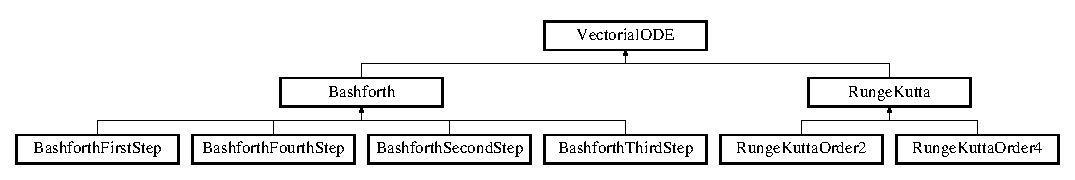
\includegraphics[height=1.971831cm]{class_vectorial_o_d_e}
\end{center}
\end{figure}
\subsection*{Public Member Functions}
\begin{DoxyCompactItemize}
\item 
\mbox{\label{class_vectorial_o_d_e_af9b113dd66c8d39473f13238cd6cb465}} 
\textbf{ Vectorial\+O\+DE} ()
\begin{DoxyCompactList}\small\item\em Constructor by default which is empty. \end{DoxyCompactList}\item 
\textbf{ Vectorial\+O\+DE} (\textbf{ Input} \&input\+\_\+object, \textbf{ Solution} \&solution\+\_\+object)
\item 
\mbox{\label{class_vectorial_o_d_e_aa4fe0065743c8c7554490b4a4e40cbe6}} 
virtual void {\bfseries Solve\+Vectorial\+O\+DE} ()=0
\item 
vector$<$ double $>$ \textbf{ Get\+Columns\+Of\+Matrix} (vector$<$ vector$<$ double $>$$>$ matrix, int position)
\begin{DoxyCompactList}\small\item\em Method allowing the access to one columns of one matrix. The chosen columns is define by the index. This method we be accessible in the inherited classes. \end{DoxyCompactList}\item 
vector$<$ vector$<$ double $>$ $>$ \textbf{ Multiply} (const vector$<$ vector$<$ double $>$$>$ \&matrix, double number)
\begin{DoxyCompactList}\small\item\em Method allowing the multiplication of a matrix with a scalar. This method we be accessible in the inherited classes. \end{DoxyCompactList}\item 
vector$<$ vector$<$ double $>$ $>$ \textbf{ Addition} (const vector$<$ vector$<$ double $>$$>$ \&matrix, double number)
\begin{DoxyCompactList}\small\item\em Method allowing the addition of a matrix with a scalar. This method we be accessible in the inherited classes. \end{DoxyCompactList}\item 
vector$<$ double $>$ \textbf{ Multiply\+With\+Vector\+By\+Right} (const vector$<$ vector$<$ double $>$$>$ \&matrix, const vector$<$ double $>$ \&matrix\+\_\+columns)
\begin{DoxyCompactList}\small\item\em Method allowing the multiplication of a matrix with a vector coming from the right side of the matrix. This method we be accessible in the inherited classes. \end{DoxyCompactList}\item 
vector$<$ double $>$ \textbf{ Multiply\+Vector\+And\+Scalar} (const vector$<$ double $>$ \&vector\+\_\+to\+\_\+multiply, double scalar)
\begin{DoxyCompactList}\small\item\em Method allowing the multiplication of a vector with a scalar. This method we be accessible in the inherited classes. \end{DoxyCompactList}\item 
vector$<$ double $>$ \textbf{ Add\+Two\+Vector} (const vector$<$ double $>$ \&vector\+\_\+1, const vector$<$ double $>$ \&vector\+\_\+2)
\begin{DoxyCompactList}\small\item\em Method allowing the addition of two vectors. This method we be accessible in the inherited classes. \end{DoxyCompactList}\item 
vector$<$ double $>$ \textbf{ Subtract\+Two\+Vector} (const vector$<$ double $>$ \&vector\+\_\+1, const vector$<$ double $>$ \&vector\+\_\+2)
\begin{DoxyCompactList}\small\item\em Method allowing the subtraction of two vectors. This method we be accessible in the inherited classes. \end{DoxyCompactList}\item 
\mbox{\label{class_vectorial_o_d_e_a17cb307ae259061b38b6e24440ae175f}} 
\textbf{ $\sim$\+Vectorial\+O\+DE} ()
\begin{DoxyCompactList}\small\item\em Destructor by default. \end{DoxyCompactList}\end{DoxyCompactItemize}
\subsection*{Protected Attributes}
\begin{DoxyCompactItemize}
\item 
\mbox{\label{class_vectorial_o_d_e_a17c81799a866e20000f436510b0c5ef4}} 
\textbf{ Input} $\ast$ {\bfseries input}
\item 
\mbox{\label{class_vectorial_o_d_e_a6b55b7c4ab7fefba07435530ba4a4ca6}} 
\textbf{ Solution} $\ast$ {\bfseries solution}
\end{DoxyCompactItemize}


\subsection{Detailed Description}
Class allowing the definition O\+DE solvers. This is an abstract class. The method Solve\+Vectorial\+O\+DE is virtual and it will be defined in different ways in the inherited classes. 

\subsection{Constructor \& Destructor Documentation}
\mbox{\label{class_vectorial_o_d_e_a9edc40bdb493be8018bdc5c5844026bb}} 
\index{Vectorial\+O\+DE@{Vectorial\+O\+DE}!Vectorial\+O\+DE@{Vectorial\+O\+DE}}
\index{Vectorial\+O\+DE@{Vectorial\+O\+DE}!Vectorial\+O\+DE@{Vectorial\+O\+DE}}
\subsubsection{Vectorial\+O\+D\+E()}
{\footnotesize\ttfamily Vectorial\+O\+D\+E\+::\+Vectorial\+O\+DE (\begin{DoxyParamCaption}\item[{\textbf{ Input} \&}]{input\+\_\+object,  }\item[{\textbf{ Solution} \&}]{solution\+\_\+object }\end{DoxyParamCaption})}

Constructor which overridden the default one. 
\begin{DoxyParams}{Parameters}
{\em input\+\_\+object} & \+: Object of \doxyref{Input}{p.}{class_input} class containing all the input informations we need to define and solve the problem. \\
\hline
{\em output\+\_\+object} & \+: Object of \doxyref{Solution}{p.}{class_solution} class containing the initialised solution matrix where we will write the results. \\
\hline
\end{DoxyParams}


\subsection{Member Function Documentation}
\mbox{\label{class_vectorial_o_d_e_a043c8b38826411e8b7cb807a59c53048}} 
\index{Vectorial\+O\+DE@{Vectorial\+O\+DE}!Addition@{Addition}}
\index{Addition@{Addition}!Vectorial\+O\+DE@{Vectorial\+O\+DE}}
\subsubsection{Addition()}
{\footnotesize\ttfamily vector$<$ vector$<$ double $>$ $>$ Vectorial\+O\+D\+E\+::\+Addition (\begin{DoxyParamCaption}\item[{const vector$<$ vector$<$ double $>$$>$ \&}]{matrix,  }\item[{double}]{number }\end{DoxyParamCaption})}



Method allowing the addition of a matrix with a scalar. This method we be accessible in the inherited classes. 


\begin{DoxyParams}{Parameters}
{\em matrix} & \+: Vector of vector of double representing the matrix we want to add. \\
\hline
{\em scalar} & \+: Integer corresponding to the scalar we want to add. \\
\hline
\end{DoxyParams}
\begin{DoxyReturn}{Returns}
Vector of vector of double (which is a matrix) corresponding to the output of the addition. 
\end{DoxyReturn}
\mbox{\label{class_vectorial_o_d_e_abb69cbfac6811f166d22a4cd394dd8fb}} 
\index{Vectorial\+O\+DE@{Vectorial\+O\+DE}!Add\+Two\+Vector@{Add\+Two\+Vector}}
\index{Add\+Two\+Vector@{Add\+Two\+Vector}!Vectorial\+O\+DE@{Vectorial\+O\+DE}}
\subsubsection{Add\+Two\+Vector()}
{\footnotesize\ttfamily vector$<$ double $>$ Vectorial\+O\+D\+E\+::\+Add\+Two\+Vector (\begin{DoxyParamCaption}\item[{const vector$<$ double $>$ \&}]{vector\+\_\+1,  }\item[{const vector$<$ double $>$ \&}]{vector\+\_\+2 }\end{DoxyParamCaption})}



Method allowing the addition of two vectors. This method we be accessible in the inherited classes. 


\begin{DoxyParams}{Parameters}
{\em vector\+\_\+1} & \+: Vector of double representing the first vector we want to add. \\
\hline
{\em vector\+\_\+2} & \+: Vector of double representing the second vector we want to add. \\
\hline
\end{DoxyParams}
\begin{DoxyReturn}{Returns}
Vector of double (which is a vector) corresponding to the output of the addition. 
\end{DoxyReturn}
\mbox{\label{class_vectorial_o_d_e_adaa675ba0b63e1c2921fb25ce5f5da57}} 
\index{Vectorial\+O\+DE@{Vectorial\+O\+DE}!Get\+Columns\+Of\+Matrix@{Get\+Columns\+Of\+Matrix}}
\index{Get\+Columns\+Of\+Matrix@{Get\+Columns\+Of\+Matrix}!Vectorial\+O\+DE@{Vectorial\+O\+DE}}
\subsubsection{Get\+Columns\+Of\+Matrix()}
{\footnotesize\ttfamily vector$<$ double $>$ Vectorial\+O\+D\+E\+::\+Get\+Columns\+Of\+Matrix (\begin{DoxyParamCaption}\item[{vector$<$ vector$<$ double $>$$>$}]{matrix,  }\item[{int}]{position }\end{DoxyParamCaption})}



Method allowing the access to one columns of one matrix. The chosen columns is define by the index. This method we be accessible in the inherited classes. 


\begin{DoxyParams}{Parameters}
{\em matrix} & \+: Vector of vector of double representing the matrix we want to access. \\
\hline
{\em position} & \+: Integer corresponding to the index of the columns of the matrix we will return. \\
\hline
\end{DoxyParams}
\begin{DoxyReturn}{Returns}
Vector of double corresponding to one columns of the matrix given by the index 
\end{DoxyReturn}
\mbox{\label{class_vectorial_o_d_e_a2d34d64b401ee86f150132e98b6a986e}} 
\index{Vectorial\+O\+DE@{Vectorial\+O\+DE}!Multiply@{Multiply}}
\index{Multiply@{Multiply}!Vectorial\+O\+DE@{Vectorial\+O\+DE}}
\subsubsection{Multiply()}
{\footnotesize\ttfamily vector$<$ vector$<$ double $>$ $>$ Vectorial\+O\+D\+E\+::\+Multiply (\begin{DoxyParamCaption}\item[{const vector$<$ vector$<$ double $>$$>$ \&}]{matrix,  }\item[{double}]{number }\end{DoxyParamCaption})}



Method allowing the multiplication of a matrix with a scalar. This method we be accessible in the inherited classes. 


\begin{DoxyParams}{Parameters}
{\em matrix} & \+: Vector of vector of double representing the matrix we want to multiply. \\
\hline
{\em scalar} & \+: Integer corresponding to the scalar we want to multiply. \\
\hline
\end{DoxyParams}
\begin{DoxyReturn}{Returns}
Vector of vector of double (which is a matrix) corresponding to the output of the multiplication. 
\end{DoxyReturn}
\mbox{\label{class_vectorial_o_d_e_a3d7e58c0622f616746ab13f5e9a7bb1c}} 
\index{Vectorial\+O\+DE@{Vectorial\+O\+DE}!Multiply\+Vector\+And\+Scalar@{Multiply\+Vector\+And\+Scalar}}
\index{Multiply\+Vector\+And\+Scalar@{Multiply\+Vector\+And\+Scalar}!Vectorial\+O\+DE@{Vectorial\+O\+DE}}
\subsubsection{Multiply\+Vector\+And\+Scalar()}
{\footnotesize\ttfamily vector$<$ double $>$ Vectorial\+O\+D\+E\+::\+Multiply\+Vector\+And\+Scalar (\begin{DoxyParamCaption}\item[{const vector$<$ double $>$ \&}]{vector\+\_\+to\+\_\+multiply,  }\item[{double}]{scalar }\end{DoxyParamCaption})}



Method allowing the multiplication of a vector with a scalar. This method we be accessible in the inherited classes. 


\begin{DoxyParams}{Parameters}
{\em vector\+\_\+to\+\_\+multiply} & \+: Vector of double representing the vector we want to multiply. \\
\hline
{\em scalar} & \+: Integer corresponding to the scalar we want to multiply. \\
\hline
\end{DoxyParams}
\begin{DoxyReturn}{Returns}
Vector of double (which is a vector) corresponding to the output of the multiplication. 
\end{DoxyReturn}
\mbox{\label{class_vectorial_o_d_e_a224a5dc0650adbf96d6274d48f629eaf}} 
\index{Vectorial\+O\+DE@{Vectorial\+O\+DE}!Multiply\+With\+Vector\+By\+Right@{Multiply\+With\+Vector\+By\+Right}}
\index{Multiply\+With\+Vector\+By\+Right@{Multiply\+With\+Vector\+By\+Right}!Vectorial\+O\+DE@{Vectorial\+O\+DE}}
\subsubsection{Multiply\+With\+Vector\+By\+Right()}
{\footnotesize\ttfamily vector$<$ double $>$ Vectorial\+O\+D\+E\+::\+Multiply\+With\+Vector\+By\+Right (\begin{DoxyParamCaption}\item[{const vector$<$ vector$<$ double $>$$>$ \&}]{matrix,  }\item[{const vector$<$ double $>$ \&}]{matrix\+\_\+columns }\end{DoxyParamCaption})}



Method allowing the multiplication of a matrix with a vector coming from the right side of the matrix. This method we be accessible in the inherited classes. 


\begin{DoxyParams}{Parameters}
{\em matrix} & \+: Vector of vector of double representing the matrix we want to multiply. \\
\hline
{\em matrix\+\_\+columns} & \+: Vector of double corresponding to the vector we want to multiply. \\
\hline
\end{DoxyParams}
\begin{DoxyReturn}{Returns}
Vector of double (which is a vector) corresponding to the output of the multiplication. 
\end{DoxyReturn}
\mbox{\label{class_vectorial_o_d_e_a0abfaf1b1fbdd1d0e7ac044da4165432}} 
\index{Vectorial\+O\+DE@{Vectorial\+O\+DE}!Subtract\+Two\+Vector@{Subtract\+Two\+Vector}}
\index{Subtract\+Two\+Vector@{Subtract\+Two\+Vector}!Vectorial\+O\+DE@{Vectorial\+O\+DE}}
\subsubsection{Subtract\+Two\+Vector()}
{\footnotesize\ttfamily vector$<$ double $>$ Vectorial\+O\+D\+E\+::\+Subtract\+Two\+Vector (\begin{DoxyParamCaption}\item[{const vector$<$ double $>$ \&}]{vector\+\_\+1,  }\item[{const vector$<$ double $>$ \&}]{vector\+\_\+2 }\end{DoxyParamCaption})}



Method allowing the subtraction of two vectors. This method we be accessible in the inherited classes. 


\begin{DoxyParams}{Parameters}
{\em vector\+\_\+1} & \+: Vector of double representing the first vector we want to subtract. \\
\hline
{\em vector\+\_\+2} & \+: Vector of double representing the second vector we want to subtract. \\
\hline
\end{DoxyParams}
\begin{DoxyReturn}{Returns}
Vector of double (which is a vector) corresponding to the output of the subtraction. 
\end{DoxyReturn}


The documentation for this class was generated from the following files\+:\begin{DoxyCompactItemize}
\item 
Vectorial\+O\+D\+E.\+h\item 
Vectorial\+O\+D\+E.\+cpp\end{DoxyCompactItemize}

%--- End generated contents ---

% Index
\backmatter
\newpage
\phantomsection
\clearemptydoublepage
\addcontentsline{toc}{chapter}{Index}
\printindex

\end{document}
